\subsection{DenseNet121}\label{s:densenet121}
\chapterauthor{Cleon Tay Shi Hong (2200649)}

DenseNet121 model is a type of convolutional neural network (CNN)\cite{Utaminingrum_Metrics_2021} architecture developed by Cornell University, This model is designed for machine learning and specifically suitable for image classification tasks. The main concept of DenseNet is to connect all layers in a feed-forward fashion, each level will get a direct input from all levels above. The DenseNet family is a set of neural architectures which are known for their densely connected structure.

\subsubsection{Implementation}

In the context of our brain tumor classification task, we employed the DenseNet121 architecture, leveraging its pretrained weights from the ImageNet dataset. This approach capitalizes on the robust feature extraction capabilities of DenseNet121 while adapting it to our specific classification requirements through further training. The DenseNet121 model was initialized with weights pretrained on ImageNet and configured to exclude its top layers, which were removed for us to customize the layers tailored for our classification task. The input images were resized to 224×224 pixels with three color channels\cite{Utaminingrum_Metrics_2021} to match the network's input specifications. This enhance the classification accuracy, ensuring that the images adhere to the network's designated input format.

Following the base layers of DenseNet121, we introduced a Global Average Pooling 2D layer. This pooling operation condenses the spatial dimensions of the feature maps into a single vector per map, enhancing computational efficiency while preserving critical features essential for classification. To mitigate overfitting, a Dropout layer with a dropout rate of 20\% was incorporated after Global Average Pooling. This layer randomly deactivates a fraction of neurons during training, promoting robustness by preventing reliance on specific neurons and facilitating the development of a more generalized model.

The classification task culminated in a Dense layer with four units\cite{Thunuguntla_S}, each corresponding to one of the brain tumor classes: meningioma, glioma, pituitary, and notumor. This layer employed a softmax activation function to produce a probability distribution across the classes, ensuring clear and interpretable classification results. For optimization, we employed the Rectified Adam optimizer (RAdam) with a learning rate of 0.0001. RAdam is known for its adaptive nature and has shown effectiveness in stabilizing training and accelerating convergence, which is particularly advantageous in complex transfer learning scenarios. The model was compiled using categorical cross-entropy loss, appropriate for multi-class classification tasks like ours. This loss function computed the discrepancy between predicted probabilities and actual class labels, guiding the model towards accurate predictions.

Training proceeded over 150 epochs with a batch size of 10, utilizing callbacks to enhance performance and prevent overfitting. Specifically, ModelCheckpoint saved the best-performing model based on validation loss, while EarlyStopping halted training when no improvement in validation loss was observed over a specified number of epochs.Upon evaluation on the test set, the DenseNet121 model achieved an impressive accuracy of 99.2\% and a validation accuracy of 87.78\%. The validation loss was recorded at 0.4012, affirming the model's robust and reliable performance across different datasets.

\subsubsection{Fine-Tuning}

In the process of refining the model for brain tumor classification, we employed a systematic approach to optimize hyperparameters critical for achieving superior performance. This fine-tuning process aimed to tailor the pretrained DenseNet121 architecture to effectively discern between different types of brain tumors.

Initially, we evaluated and explored three different optimizers: RAdam\cite{Tanner_2021}, Adam, and SGD, aiming to identify the most effective one for our specific task. The pretrained DenseNet121 model was adapted with additional layers, and each optimizer was evaluated based on its ability to improve validation accuracy during training.

After comprehensive experimentation and comparative analysis, RAdam emerged as the optimal choice. RAdam consistently outperformed Adam and SGD in terms of achieving higher validation accuracy. This selection aligns with research findings, which emphasize RAdam's advantages in stabilizing training dynamics and accelerating convergence rates, particularly in complex transfer learning scenarios like ours.

\subsubsection{Results and Evaluation}

\begin{figure}[H]
  \centering
  \begin{subfigure}[b]{0.2\textwidth}
    \centering
    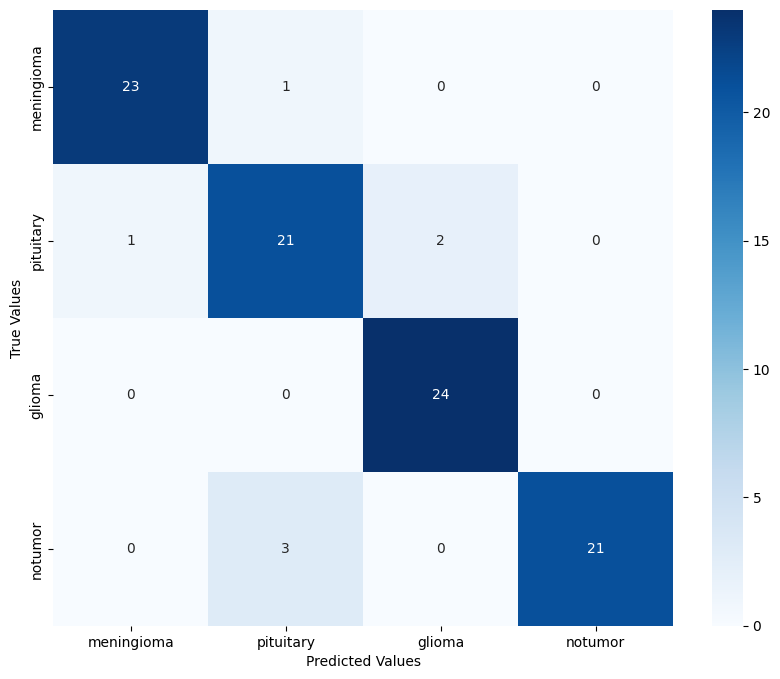
\includegraphics[width=\textwidth]{densenet121/evaluation/cm1.png}
    \caption{Confusion Matrix}
    \label{fig:densenet121_cm1}
  \end{subfigure}
  \hfill
  \begin{subfigure}[b]{0.2\textwidth}
    \centering
    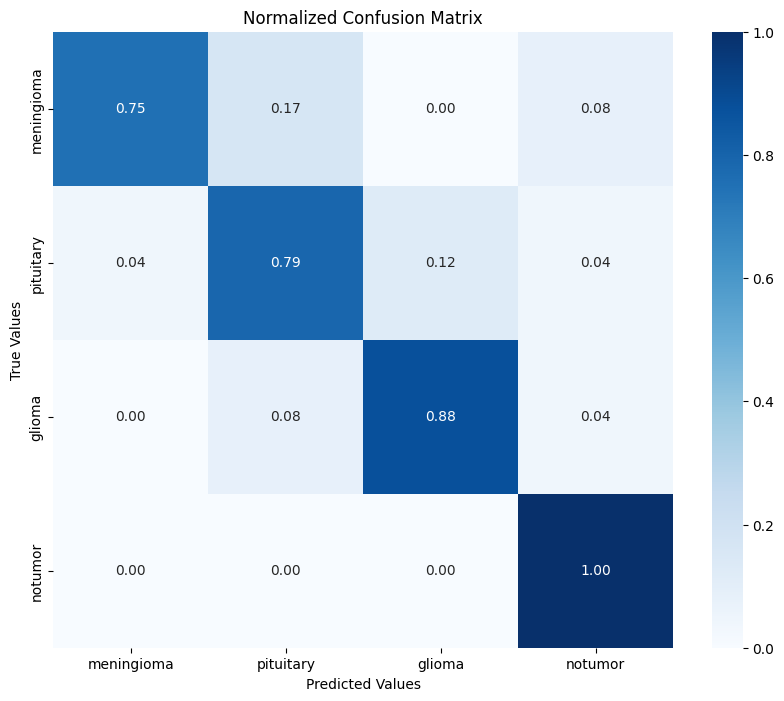
\includegraphics[width=\textwidth]{densenet121/evaluation/cm2.png}
    \caption{Normalized Confusion Matrix}
    \label{fig:densenet121_cm2}
  \end{subfigure}
  \hfill
  \begin{subfigure}[b]{0.25\textwidth}
    \centering
    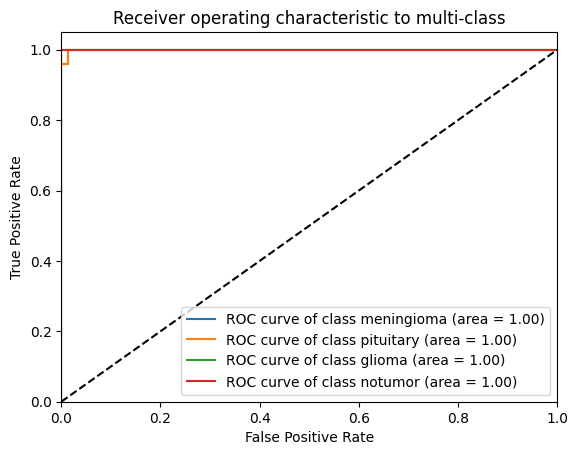
\includegraphics[width=\textwidth]{densenet121/evaluation/ROC.png}
    \caption{ROC Curve}
    \label{fig:densenet121_roc}
  \end{subfigure}
  \hfill
  \begin{subfigure}[b]{0.25\textwidth}
    \centering
    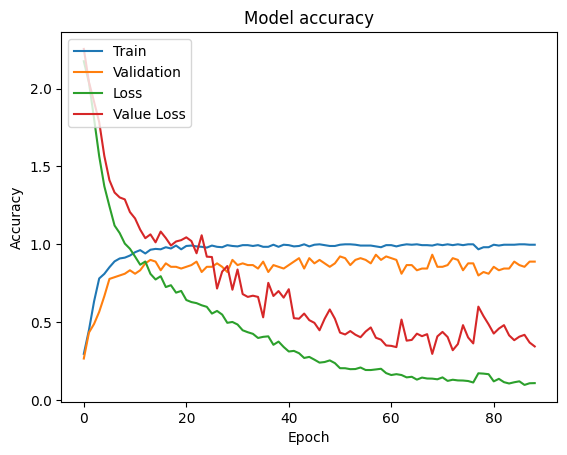
\includegraphics[width=\textwidth]{densenet121/evaluation/learning_curve.png}
    \caption{Learning Curve}
    \label{fig:densenet121_learning_curve}
  \end{subfigure}
  \caption{Confusion Matrix, Normalized Confusion Matrix, ROC Curve, and Learning Curve for Brain Tumor Segmentation}
  \label{fig:densenet121_evaluation}
\end{figure}

\begin{table}[ht]
\centering
\begin{tabular}{cc}
    \begin{minipage}{.6\linewidth}
        \centering
        \begin{subtable}[t]{\linewidth}
            \centering
            \begin{tabular}{|l|c|c|c|c|}
                \hline 
                \textbf{Class} & \textbf{Precision} & \textbf{Recall} & \textbf{F1-Score} & \textbf{Support} \\ 
                \hline 
                meningioma & 0.82 & 0.75 & 0.78 & 24 \\ 
                \hline
                pituitary  & 0.92 & 0.96 & 0.94 & 24 \\ 
                \hline
                glioma     & 0.95 & 0.83 & 0.89 & 24 \\ 
                \hline
                notumor    & 0.82 & 0.96 & 0.88 & 24 \\ 
                \hline
                micro avg  & 0.88 & 0.88 & 0.88 & 96 \\ 
                \hline
                macro avg  & 0.88 & 0.88 & 0.87 & 96 \\ 
                \hline
                weighted avg & 0.88 & 0.88 & 0.87 & 96 \\ 
                \hline
                samples avg & 0.88 & 0.88 & 0.88 & 96 \\ 
                \hline
            \end{tabular}
            \caption{Classification Report for Brain Tumor Segmentation} 
            \label{tab:densenet121_classification_report}
        \end{subtable}
    \end{minipage} &
    \begin{minipage}{.35\linewidth}
        \centering
        \begin{subtable}[t]{\linewidth}
            \centering
            \begin{tabular}{|c|c|}
                %DSC: 0.8737221198401323, Sensitivity: 0.8750000000000001, Specificity: 0.9583333333333334, Accuracy: 0.875
                \hline 
                \textbf{Metric} & \textbf{Value} \\ 
                \hline
                DSC & 0.8737 \\ 
                \hline
                Sensitivity & 0.8750 \\ 
                \hline
                Specificity & 0.9583 \\ 
                \hline
                Accuracy & 0.8750 \\ 
                \hline
            \end{tabular}
            \caption{Additional Metrics for Brain Tumor Segmentation} 
            \label{tab:densenet121_additional_metrics}
        \end{subtable}
    \end{minipage}
\end{tabular}
\caption{Classification Report and Additional Metrics for Brain Tumor Segmentation using DenseNet121}
\label{tab:combined_densenet121_metrics}
\end{table}

In Figures \ref{fig:densenet121_cm1} and \ref{fig:densenet121_cm2} shows the confusion matrices, it provide a descriptive view of the model's performance on classifying the four brain tumor classes: meningioma, pituitary, glioma, and no tumor. The meningioma and glioma classes exhibit lower rates but still commendable true positive percentage of 75\% and 83\% respectively. The classification report in Table \ref{tab:densenet121_classification_report} summarizes the precision, recall, and F1-score for each class. DenseNet121 model shows average precision and recall across all classes, having F1-score of 0.94 for the pituitary class. The overall micro and sample averages for precision, recall, and F1-score stood at 0.88 while the overall micro and weighted averages for precision, recall, and F1-score all stand at 0.87, reflecting consistent and reliable performance.

The ROC curve in Figure \ref{fig:densenet121_roc} displays the true positive rate against the false positive rate for each class. The areas under the curve (AUC) for pituitary class is perfect at 1.00, while notumor and glioma classes show AUCs of 0.99 and meningioma AUCs at 0.95. indicating excellent discriminative ability of the model.

The learning curve in Figure \ref{fig:densenet121_learning_curve} provides valuable insights into how the model learns and improves over time, offering a visual representation of key metrics such as training and validation accuracy and loss over 150 epochs. The alignment between training and validation accuracy, coupled with the consistent decrease in loss values, suggests that the model has effectively learned from the data without exhibiting notable signs of overfitting.

Table \ref{tab:densenet121_additional_metrics} presents key performance metrics for the model, including the Dice Similarity Coefficient (DSC), sensitivity, specificity, and accuracy. The model achieved a DSC of 0.8737, indicating substantial overlap between predicted and actual tumor regions. Sensitivity and accuracy, both measuring 0.8750, highlight the model's proficiency in correctly identifying true positives. Additionally, a specificity of 0.9583 demonstrates its effectiveness in accurately identifying true negatives. These metrics collectively underscore the model's strong performance in brain tumor segmentation.

\subsubsection{K-Folds Cross-Validation}

\begin{figure}[H]
  \begin{center}
    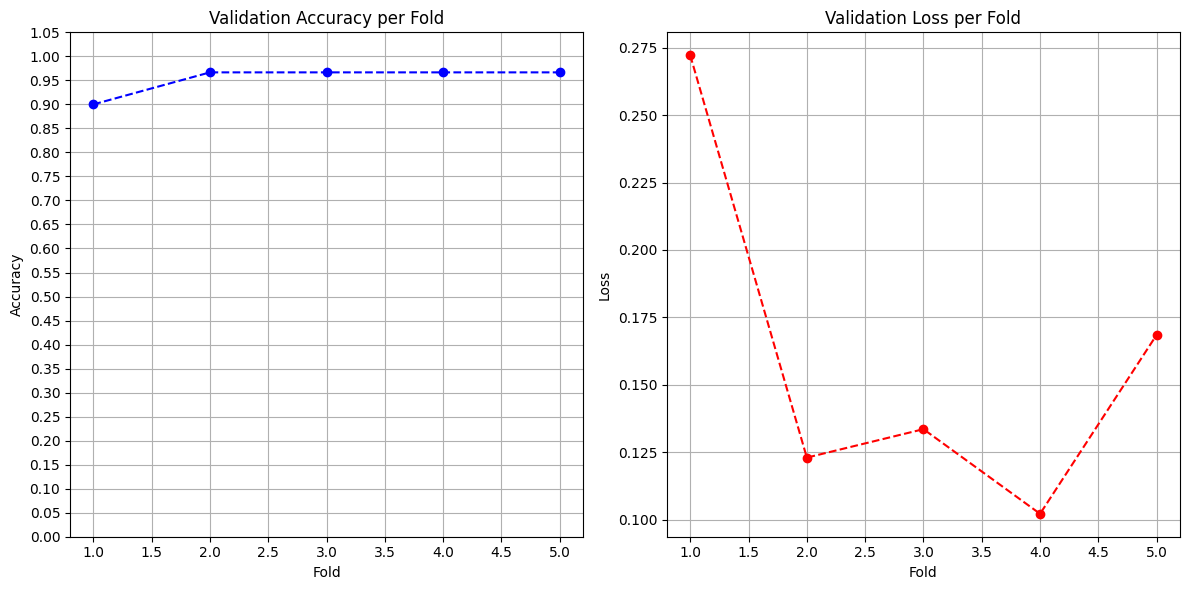
\includegraphics[width=0.7\textwidth]{densenet121/evaluation/kfolds.png}
  \end{center}
  \caption{K-Folds Cross-Validation for Brain Tumor Segmentation}\label{f:densenet121_kfolds}
\end{figure}

K-Folds cross-validation was utilized to comprehensively assess the model's performance across diverse subsets of the dataset. This method divides the dataset into $k$ equal parts, or folds, where the model is trained on $k−1$ folds and validated on the remaining fold in each iteration. This process is repeated $k$ times, ensuring that each fold serves as the validation set exactly once. By averaging the validation accuracy and loss metrics across all folds, we obtain a robust measure of the model's performance and its ability to generalize to unseen data.

Table \ref{tab:densenet121_kfolds_metrics} summarizes the outcomes of the K-Folds cross-validation, presenting average values and standard deviations of key metrics. The results demonstrate consistent performance across all folds, with minimal variance in accuracy and loss values. This consistency underscores the model's reliability and effectiveness in accurately segmenting brain tumors.

The setup for K-Folds cross-validation is detailed in Table \ref{tab:densenet121_kfolds_conditions}, specifying the parameters chosen to ensure thorough training and robust evaluation of the model. These settings were carefully selected to validate the model's performance comprehensively and reliably across different subsets of the dataset.

\begin{table}[H]
\centering
\caption{K-Folds Cross-Validation Testing Conditions}\label{tab:densenet121_kfolds_conditions}
\begin{tabular}{cc}
    \begin{minipage}{.45\linewidth}
        \centering
        \begin{subtable}[t]{\linewidth}
            \centering
            \begin{tabular}{|l|c|}
                \hline
                \textbf{Parameter} & \textbf{Value} \\
                \hline
                Number of Folds ($k$) & 5 \\
                \hline
                Epochs & 90 \\
                \hline
                Batch Size & 10 \\
                \hline
            \end{tabular}
            \caption{Training Parameters}
            \label{tab:densenet121_kfolds_parameters}
        \end{subtable}
    \end{minipage} &
    \begin{minipage}{.45\linewidth}
        \centering
        \begin{subtable}[t]{\linewidth}
            \centering
            \begin{tabular}{|l|c|}
                \hline
                \textbf{Metric} & \textbf{Value} \\
                \hline
                Average Validation Accuracy & 0.9630 \\
                \hline
                Average Validation Loss & 0.2230 \\
                \hline
                Validation Accuracy Std. Dev. & 0.0263 \\
                \hline
                Validation Loss Std. Dev. & 0.0785 \\
                \hline
            \end{tabular}
            \caption{Evaluation Metrics}
            \label{tab:densenet121_kfolds_metrics}
        \end{subtable}
    \end{minipage}
\end{tabular}
\end{table}

The outcomes derived from K-Folds cross-validation underscore the model's robustness and dependability in classifying brain tumor images. With minimal variability in accuracy and loss metrics, the results affirm that the model effectively generalizes across diverse data subsets. This capability mitigates concerns of overfitting, ensuring reliable performance suitable for real-world applications.

% Validation Accuracy: 0.9630 ± 0.0370
% Validation Loss: 0.2230 ± 0.7770
% k = 5
% epochs = 90 
% batch_size = 10


\subsubsection{Conclusion}

The implemented DenseNet121 model leverages the powerful architecture pretrained on ImageNet, has been successfully applied in brain tumor segmentation tasks. By harnessing transfer learning and fine-tuning techniques, the DenseNet121 model adapts its feature extraction capabilities to our specific brain tumor classification task. This approach ensures that the model benefits from learned features relevant to medical imaging, enhancing its ability to classify brain tumor images accurately. Moreover, the choice of the Rectified Adam optimizer facilitates efficient training and convergence. The performance of the model has been rigorously validated through techniques like K-Folds cross-validation, demonstrating robustness and consistency across diverse subsets of our dataset. This validation underscores the model's reliability and potential for clinical applications in diagnosis and treatment planning, making it a valuable tool in medical imaging.
